\documentclass[11pt,titlepage,a4paper]{article}
\newcommand{\HRule}{\rule{\linewidth}{0.5mm}}
\usepackage{graphicx}
\begin{document}


\begin{titlepage}
\begin{center}

\textsc{\LARGE School of Computing,University of Utah}\\[1.5cm]

\textsc{\Large Independent Study Report}\\[0.5cm]

% Title
\HRule \\[0.4cm]
{ \huge \bfseries UserSpace Device Access in Linux \\[0.4cm] }

\HRule \\[1.5cm]

% Author and supervisor
\begin{minipage}{0.4\textwidth}
\begin{flushleft} \large
\emph{Author:}\\
Sriraam \textsc{Appusamy Subramanian}
\end{flushleft}
\end{minipage}
\begin{minipage}{0.4\textwidth}
\begin{flushright} \large
\emph{Supervisor:} \\
Robert Ricci \\
Anton Burtsev
\end{flushright}
\end{minipage}

\vfill

% Bottom of the page
{\large \today}

\end{center}
\end{titlepage}

\begin{abstract}
Operating system allows processes in the system to share the computing, storage and peripheral resources with safety and isolation. Much of the mechanisms involved in achieving the above capabilities trades off performance/latency for flexibility which remains acceptable for most of the day-to-day applications. However,for certain applications like memcached, SDN controller,etc., whose performance is tied to their disk/peripheral device access capabilities, this flexibility is less desirable than performance. The goal of this independent study was to evaluate and explore existing systems that allow for direct peripheral device assignment to applications, exclusive or not.Intel's DataPlane Development Kit (DPDK) is a software library that uses modified userspace drivers, polling, prefetching/pre-allocation of buffers/queues and other enhancements to allow upto 80Mpps packet processing capabilities on Intel Architecture platforms. However DPDK supports restrictive number of NIC types.  Intel VT-d is an hardware virtualization technique that provides dedicated I/O Memory management unit and Interrupt remapping capabilities that could allow for exclusive device usage by an application. SUD is an existing system, developed using Usermode Linux(UML) that aims to test malicious device drivers by running them in userspace. Since SUD was implemented in linux kernel 2.6.x, it became necessary to port the project to linux kernel 3.10.x to allow for further testing and benchmarking. Although most of the porting is done, testing still remains incomplete due to failed porting of broadcom driver BNX2 into UMLinux. 
\end{abstract}

\section{DPDK}
Intel's DataPlane Development Kit aims to improve packet processing performance in Intel platforms. This is achieved by providing applications with customized software library that significantly improves peripheral device access performance. This library provides a simple API interface for buffer management, queue management, poll-mode capable userspace drivers and packet-flow classification. Further several abstraction layers are added to both userspace and kernel-space to help communicate with the peripheral device in traditional Linux-based operating systems. An experiment was setup in Emulab with gpu2 node and 2 Network Interace Cards(NICs) were assigned to DPDK. Following this, a sample application was run to verify DPDK. After a quick analysis of the existing openflow controllers and their performance metrics, NOX was chosen to be modified to support DPDK. However,limited types of hardware supported by DPDK warranted continued exploration for other mechanisms.
\section{SUD}
SUD is a system that aims to protect system resources against potentially malicious device drivers. This is achieved by moving the device driver out of the kernel-space and using User Mode Linux (UMLinux) to provide access to hardware features. In this system, a safe and generic proxy driver is added for each class of peripheral device. This proxy driver registers itself to the kernel as the device driver for the device of interest. A Message passing mechanism is setup between the proxy driver and the unmodified driver running in the userspace. This bidirectional message passing is supplemented by PCIe emulation and Message Signalling Interrupts(MSI) to provide safe access to devices. Further, SUD relies on reading/writing physical memory via DMA, a capability allowed by IOMMU (Intel or AMD) that supports isolation and memory mapped I/O for certain devices.
\section{Porting to 3.x kernel}
The primary task was to port the implementation of SUD to currently used linux kernel versions i.e. 3.10.x. This task involved modifying the linux kernel to add proxy driver and other patches. The port was performed to a d710 node in Emulab that has 4 Broadcom NetXtreme II BCM5709 Gigabit Ethernet chipsets. Following this, UMLinux was  built with PCI emulation and unmodified device driver.Much of the implementation was ported directly to the new kernel with significant number of tweaks for compatibility. Although PCI emulation feature port was direct, recent broadcom device driver port in UMLinux has been so far unsuccessful since the device driver is more recent than the substrate it integrates with. One approach might be to use an older version of the device driver. However, this remains untested and just a temporary solution.
\section{Results}
The SUD port was almost nearly complete with proxy driver(ud\_net) being registered in the host kernel. The UMLinux device driver process was compiled without the necessary broadcom device driver and so it could not be thoroughly tested. However the following screenshots show the status,in detail. 

\begin{figure}[h!]
  \caption{UMLinux device driver process, waiting on events}
  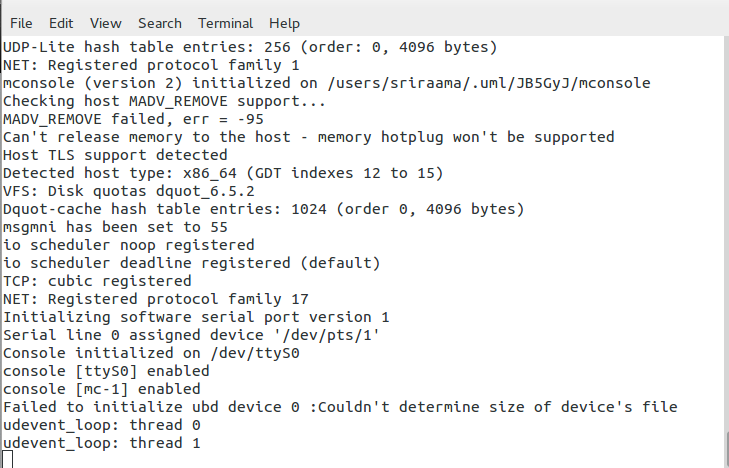
\includegraphics[width=0.75\textwidth]{./scr.png}
\end{figure}
\begin{figure}[h!]
  \caption{Host kernel 'lspci -k' showing the ud\_net proxy driver registered for NICs}
  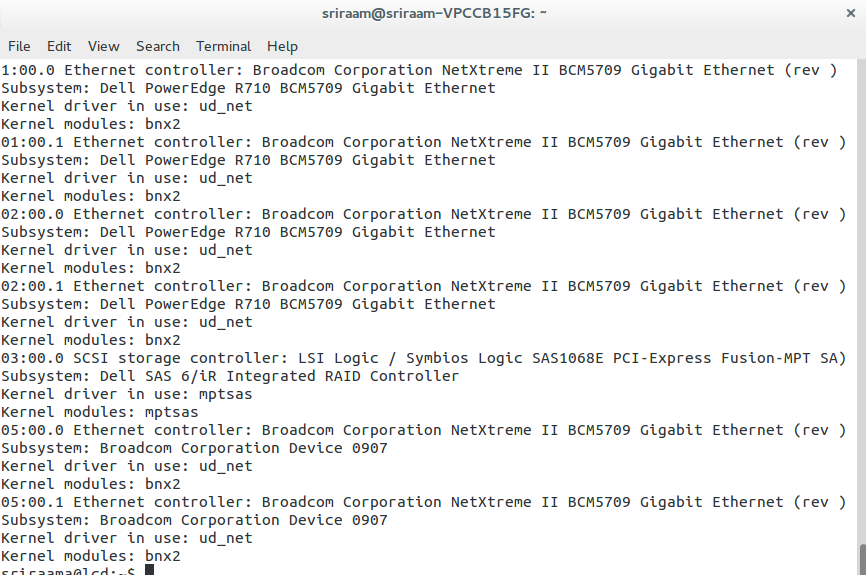
\includegraphics[width=0.75\textwidth]{./ud.png}
\end{figure}


\section{Conclusion}
Although porting SUD from older to newer kernel version was exhausting and tedious, it provided great insight into programming IOMMU and device drivers ,proving to be a rich learning experience. In retrospect, it might have been better to build SUD for the recent linux kernel from  scratch, with support for newer features  might have been a rewarding experience. 

\end{document}
